\documentclass[aspectratio=169,notes]{beamer}
\usepackage{lmodern}
\usepackage{adjustbox}
\usepackage[T1]{fontenc}
\usepackage{textcomp}
\usepackage{animate}
\usepackage{underscore}
\usepackage{pdfpc-commands}
\usepackage{xmpmulti}
\usepackage{multimedia}
\usepackage{epstopdf}
\usepackage{bbding}
\usepackage[absolute,overlay]{textpos}
\usepackage[most]{tcolorbox}
%\usepackage{ctex}

\definecolor{Title}{rgb}{0.94,0.52,0.08}
\setbeamercolor{frametitle}{bg=Title,fg=black}

% footnote without number
\makeatletter
\def\blfootnote{\xdef\@thefnmark{}\@footnotetext}
\makeatother

\newcommand\Wider[2][3em]{%
\makebox[\linewidth][c]{%
  \begin{minipage}{\dimexpr\textwidth+#1\relax}
  \raggedright#2
  \end{minipage}%
  }%
}

\usepackage{hyperref}
\usepackage{scalerel}
\def\thumbup{\scalerel*{\includegraphics{thumbup.png}}{O}}
\usepackage{listings}
\lstdefinelanguage{D}
{
  % list of keywords
  morekeywords={ abstract, alias, align, asm, assert, auto, body, bool, break,
	byte, case, cast, catch, cdouble, cent, cfloat, char, class, const,
	continue, default, double, else, enum, export, extern, false, final, finally,
	float, for, foreach, foreach_reverse, function, goto, idouble, if, ifloat,
	immutable, import, in, inout, int, interface, invariant, ireal, is, lazy,
	long, mixin, module, new, nothrow, null, out, override, package, pragma,
	private, protected, public, pure, real, ref, return, scope, shared, short,
	static, string, struct, super, switch, synchronized, template, this, throw,
	true, try, typeid, typeof, ubyte, ucent, uint, ulong, union,
	unittest, delegate, @safe, @property, @trusted,
	ushort, version, void, wchar, while, with, __FILE__, __FILE_FULL_PATH__,
	__MODULE__, __LINE__, __FUNCTION__, __PRETTY_FUNCTION__, __gshared,
	__traits, __vector, __parameters
  },
  otherkeywords= { @property, @safe },
  sensitive=false, % keywords are not case-sensitive
  morecomment=[l]{//}, % l is for line comment
  morecomment=[s]{/*}{*/}, % s is for start and end delimiter
  morecomment=[s]{/+}{+/}, % s is for start and end delimiter
  morestring=[b]{"}, % defines that strings are enclosed in double quotes
  morestring=[b]{`} % defines that strings are enclosed in double quotes
}
\usepackage{color}
\definecolor{eclipseBlue}{RGB}{42,0.0,255}
\definecolor{eclipseGreen}{RGB}{63,127,95}
\definecolor{eclipsePurple}{RGB}{127,0,85}

% Set Language
\lstset{
  language={D},
  basicstyle=\small\ttfamily, % Global Code Style
  captionpos=b, % Position of the Caption (t for top, b for bottom)
  extendedchars=true, % Allows 256 instead of 128 ASCII characters
  tabsize=2, % number of spaces indented when discovering a tab 
  columns=fixed, % make all characters equal width
  keepspaces=true, % does not ignore spaces to fit width, convert tabs to spaces
  showstringspaces=false, % lets spaces in strings appear as real spaces
  breaklines=true, % wrap lines if they don't fit
  numbers=left, % show line numbers at the left
  numberstyle=\tiny\ttfamily, % style of the line numbers
  commentstyle=\color{eclipseGreen}, % style of comments
  keywordstyle=\color{eclipsePurple}, % style of keywords
  stringstyle=\color{eclipseBlue}, % style of strings
}
\definecolor{lightgray}{rgb}{.9,.9,.9}
\definecolor{darkgray}{rgb}{.4,.4,.4}
\definecolor{purple}{rgb}{0.65, 0.12, 0.82}
\lstdefinelanguage{TypeScript}{
	keywords={break, case, catch, continue, debugger, default, delete, do, else,
		false, from, finally, for, function, if, in, instanceof, new, null, return, switch,
		this, throw, true, try, typeof, var, void, while, with, interface,
		class, export, boolean, throw, implements, import, this, const, let,
		of, =>},
	morecomment=[l]{//},
	morecomment=[s]{/*}{*/},
	morestring=[b]',
	morestring=[b]",
	ndkeywords={},
	keywordstyle=\color{blue}\bfseries,
	ndkeywordstyle=\color{darkgray}\bfseries,
	identifierstyle=\color{black},
	commentstyle=\color{purple}\ttfamily,
	stringstyle=\color{red}\ttfamily,
	sensitive=true
}

\colorlet{punct}{red!60!black}
\definecolor{background}{HTML}{EEEEEE}
\definecolor{delim}{RGB}{20,105,176}
\colorlet{numb}{magenta!60!black}

\lstdefinelanguage{GraphQL}{
    basicstyle=\normalfont\ttfamily,
    numbers=left,
    stepnumber=1,
    showstringspaces=false,
    breaklines=true,
	keywords={type, schema, mutation, subscription, __type, __schema, kind,
		on, fragment, query},
    literate=
     *{0}{{{\color{numb}0}}}{1}
      {1}{{{\color{numb}1}}}{1}
      {2}{{{\color{numb}2}}}{1}
      {3}{{{\color{numb}3}}}{1}
      {4}{{{\color{numb}4}}}{1}
      {5}{{{\color{numb}5}}}{1}
      {6}{{{\color{numb}6}}}{1}
      {7}{{{\color{numb}7}}}{1}
      {8}{{{\color{numb}8}}}{1}
      {9}{{{\color{numb}9}}}{1}
      {:}{{{\color{punct}{:}}}}{1}
      {,}{{{\color{punct}{,}}}}{1}
      {\{}{{{\color{delim}{\{}}}}{1}
      {\}}{{{\color{delim}{\}}}}}{1}
      {[}{{{\color{delim}{[}}}}{1}
      {]}{{{\color{delim}{]}}}}{1},
}

\lstdefinelanguage{json}{
    basicstyle=\normalfont\ttfamily,
    numbers=left,
    stepnumber=1,
    showstringspaces=false,
    breaklines=true,
    literate=
     *{0}{{{\color{numb}0}}}{1}
      {1}{{{\color{numb}1}}}{1}
      {2}{{{\color{numb}2}}}{1}
      {3}{{{\color{numb}3}}}{1}
      {4}{{{\color{numb}4}}}{1}
      {5}{{{\color{numb}5}}}{1}
      {6}{{{\color{numb}6}}}{1}
      {7}{{{\color{numb}7}}}{1}
      {8}{{{\color{numb}8}}}{1}
      {9}{{{\color{numb}9}}}{1}
      {:}{{{\color{punct}{:}}}}{1}
      {,}{{{\color{punct}{,}}}}{1}
      {\{}{{{\color{delim}{\{}}}}{1}
      {\}}{{{\color{delim}{\}}}}}{1}
      {[}{{{\color{delim}{[}}}}{1}
      {]}{{{\color{delim}{]}}}}{1},
}
\usepackage{tikz}
\usetikzlibrary{shadows,calc}
\usepackage{xkeyval}
\usepackage{todonotes}
\presetkeys{todonotes}{inline}{}
\defbeamertemplate{description item}{align left}{\insertdescriptionitem\hfill}
\usetheme{metropolis}					 % Use metropolis theme
\usepackage[
    backend=biber,
	sorting=none,
    url=true 
]{biblatex}
\addbibresource{biblio.bib}
\setbeamertemplate{bibliography item}{\insertbiblabel}

\title{Simple @safe D}
\date{DConf 2023}
\author{Dr.\,Robert Schadek}

\begin{document}
	\maketitle
	\subtitle{How to make enemies quickly}
	\maketitle

	\begin{frame}[fragile]{The Problem 1/2}
		\lstinputlisting[language=D,firstnumber=1,firstline=4,lastline=17,basicstyle=\footnotesize\ttfamily]{code.d}
	\end{frame}

	\begin{frame}[fragile]{The Problem 2/2}
		\begin{itemize}
			\item Just look at all the syntax
			\item DIP1035 -- \lstinline|@system| Variables ... 
		\end{itemize}
		\pause
		\begin{itemize}	
			\item Thinking that D is the C/C++ successor ... it is not, that is rust
			\item Thinking \lstinline|@safe| languages are the new thing ...
				they are not. Most languages are safe already, python, JS, java
		\end{itemize}
	\end{frame}

	\begin{frame}[plain]{Memory safety in C++77}
		\Wider{
		\begin{tabular}{c c c}
			\includegraphics[height=0.22\paperwidth]{cpp1.png} &
			\includegraphics[height=0.22\paperwidth]{cpp2.png} &
			\includegraphics[height=0.22\paperwidth]{cpp4.png}
		\end{tabular}
		\begin{center}
		\begin{tabular}{c c}
			\includegraphics[height=0.22\paperwidth]{cpp5.png} &
			\includegraphics[height=0.22\paperwidth]{cpp6.png}
		\end{tabular}
		\end{center}
		}
	\end{frame}

	\begin{frame}[plain]{Memory safety in C++77}
		\includegraphics[width=0.86\paperwidth]{cpp7.png}
	\end{frame}


	\section{Hopefully, there are still some people in the room with me at this point}

	\begin{frame}[fragile]{DIP1000}
		\begin{columns}[T]
		\begin{column}{0.49\textwidth}
		\lstinputlisting[language=D,firstnumber=1,firstline=20,lastline=40,basicstyle=\scriptsize\ttfamily]{code.d}
		\end{column}
		\begin{column}{0.49\textwidth}
		\lstinputlisting[language=D,firstnumber=1,firstline=41,lastline=50,basicstyle=\scriptsize\ttfamily]{code.d}
		\end{column}
		\end{columns}
	\end{frame}

	\begin{frame}[fragile]{The Solution}
		\begin{itemize}
			\item instead of adding things ... lets remove things\vspace{1cm}
			\pause
			\item old school \lstinline|@safe|
			\item No unary \lstinline|&| --- remove this from the grammar in \lstinline|@safe|
			\item No \lstinline@return@ by \lstinline@ref@
			\item No slicing of static arrays
		\end{itemize}
	\end{frame}

	\begin{frame}[fragile]{The Consequences}
		\begin{itemize}
			\item No need for DIP1000, DIP1021, and DIP 1035
			\item No user defined \lstinline|@safe| container that behave like in-builds
			\item No Manual Memory Management (MMM) in \lstinline|@safe| code
			\item Clear definition of \lstinline|@property|
			\item etc...
		\end{itemize}
	\end{frame}

	\section{Consequences and Remedies}

	\begin{frame}[fragile]{Passing data down}
		\begin{columns}[T]
		\begin{column}{0.49\textwidth}
		\lstinputlisting[language=D,basicstyle=\ttfamily]{refdown.d}
		\end{column}
		\pause
		\begin{column}{0.49\textwidth}
		\lstinputlisting[language=D,basicstyle=\ttfamily]{refdown2.d}
		\end{column}
		\end{columns}
	\end{frame}

	\begin{frame}[fragile]{Passing data up}
		\begin{columns}[T]
		\begin{column}{0.49\textwidth}
		\lstinputlisting[language=D,basicstyle=\ttfamily]{refup.d}
		\end{column}
		\pause
		\begin{column}{0.49\textwidth}
		\lstinputlisting[language=D,basicstyle=\ttfamily]{refup2.d}
		\end{column}
		\end{columns}
	\end{frame}

	\begin{frame}[fragile]{Container}
		\lstinputlisting[language=D,,firstnumber=1,firstline=28,lastline=34,basicstyle=\small\ttfamily]{containerref.d}
	\end{frame}

	\begin{frame}[fragile]{returning ref}
		\begin{columns}[T]
		\begin{column}{0.49\textwidth}
		\lstinputlisting[language=D,basicstyle=\scriptsize\ttfamily]{container.d}
		\end{column}
		\pause
		\begin{column}{0.49\textwidth}
		\lstinputlisting[language=D,basicstyle=\scriptsize\ttfamily]{containerref2.d}
		\end{column}
		\end{columns}
	\end{frame}

	\begin{frame}[fragile]{returning ref}
		\begin{columns}[T]
		\begin{column}{0.49\textwidth}
		\lstinputlisting[language=D,firstnumber=1,firstline=1,lastline=16,basicstyle=\scriptsize\ttfamily]{containerref.d}
		\end{column}
		\pause
		\begin{column}{0.49\textwidth}
		\lstinputlisting[language=D,,firstnumber=18,firstline=18,lastline=26,basicstyle=\scriptsize\ttfamily]{containerref.d}
		\end{column}
		\end{columns}
	\end{frame}

	\begin{frame}[fragile]{\lstinline|@property| what do you even get?}
		\lstinputlisting[language=D,basicstyle=\ttfamily]{property.d}
	\end{frame}

	\begin{frame}[fragile]{not being smart}
		\begin{columns}[T]
		\begin{column}{0.49\textwidth}
		\lstinputlisting[language=D,firstnumber=1,firstline=1,lastline=11,basicstyle=\scriptsize\ttfamily]{notsmart.d}
		\end{column}
		\begin{column}{0.49\textwidth}
		\lstinputlisting[language=D,firstnumber=13,firstline=13,basicstyle=\scriptsize\ttfamily]{notsmart.d}
		\end{column}
		\end{columns}
	\end{frame}

	\begin{frame}[plain]
  		\begin{textblock*}{0cm}(-0mm,5mm)
		\hspace{-5mm}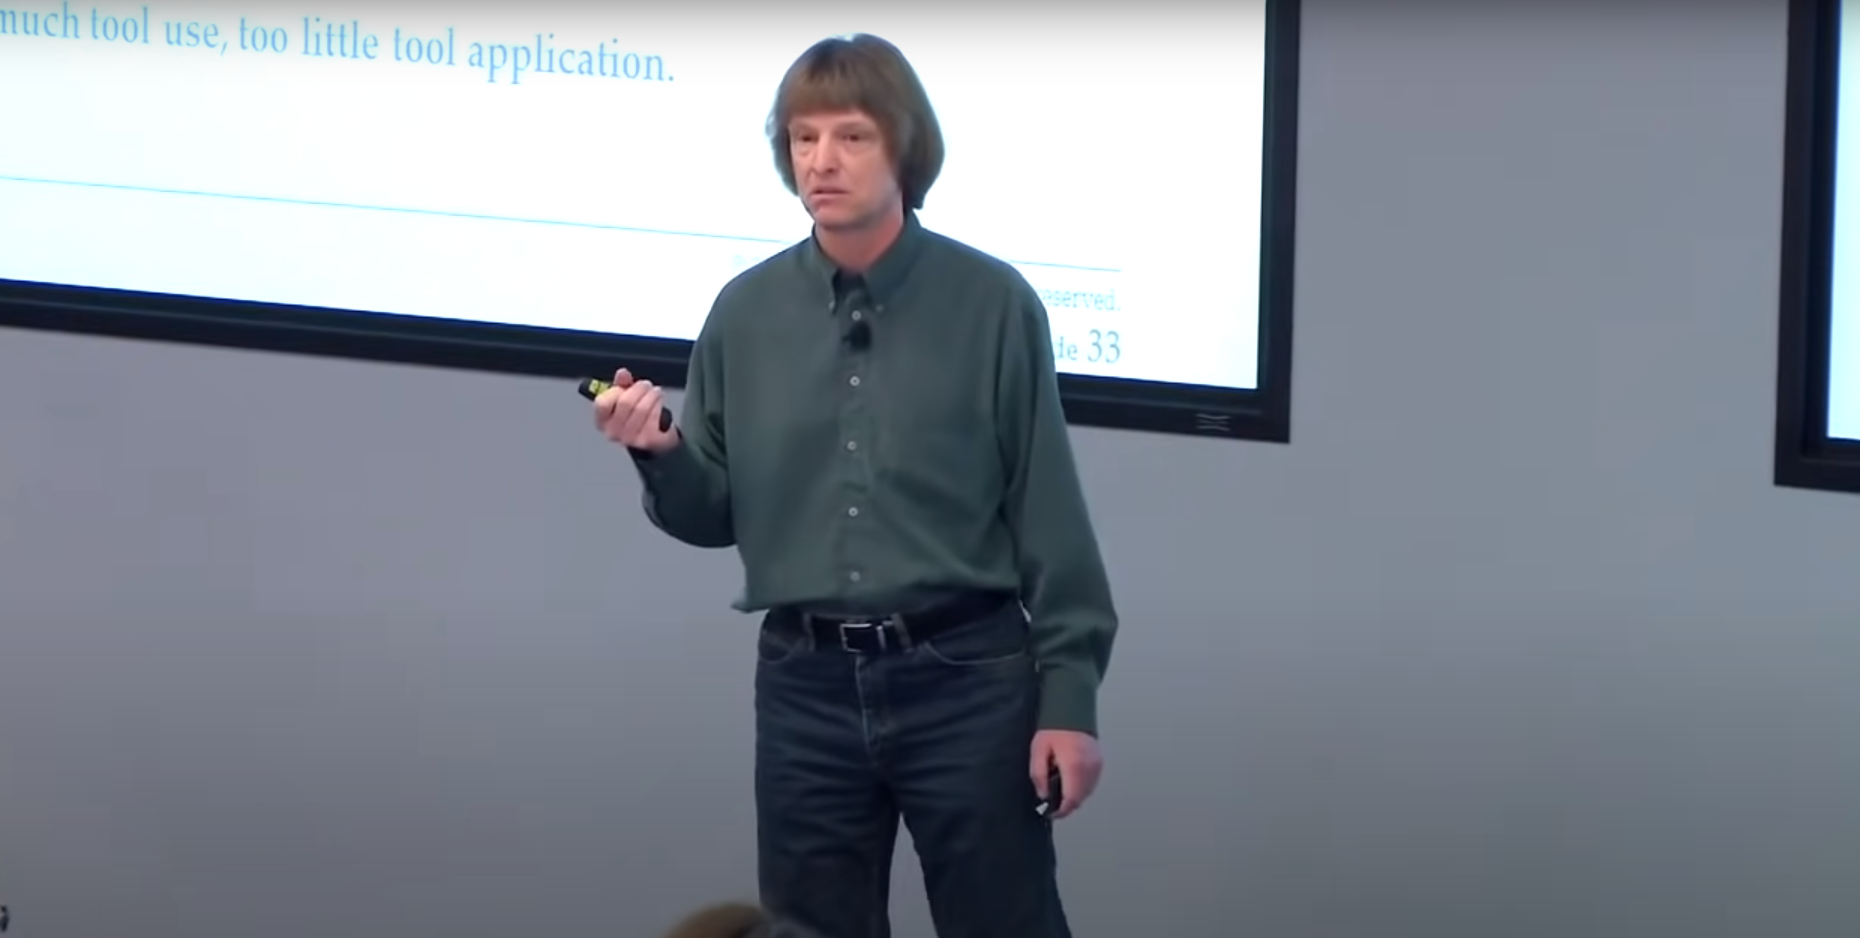
\includegraphics[width=\paperwidth]{scott.png}
		\end{textblock*}
	\end{frame}

	\section{Continuations}

	\begin{frame}[t]
		\frametitle{\lstinline@assert@s}
		\begin{columns}[T]
		\begin{column}{0.49\textwidth}
		\lstinputlisting[language=D,firstnumber=1,firstline=1,lastline=17,basicstyle=\scriptsize\ttfamily]{asserttest.d}
		\end{column}
		\begin{column}{0.49\textwidth}
		\lstinputlisting[language=D,firstnumber=19,firstline=19,basicstyle=\scriptsize\ttfamily]{asserttest.d}
		\begin{itemize}
			\item \lstinline@dmd -release -run asserttest.d@
			\item echo \$?
			\pause
			 \vspace{10mm}\item No assert, in/out contrast, or invariant
		\end{itemize}
		\end{column}
		\end{columns}
	\end{frame}

	\begin{frame}[t]
		\frametitle{Template Constraints}
		\lstinputlisting[language=D,firstnumber=1,firstline=9,lastline=23,basicstyle=\scriptsize\ttfamily]{templateconstraints.d}
	\end{frame}

	\begin{frame}[t]
		\frametitle{Template Constraints continued}
		\lstinputlisting[language=D,firstnumber=15,firstline=24,lastline=38,basicstyle=\scriptsize\ttfamily]{templateconstraints.d}
	\end{frame}

	\begin{frame}[t]
		\frametitle{Template Constraints continued}
		\lstinputlisting[language=D,firstnumber=30,firstline=39,lastline=51,basicstyle=\scriptsize\ttfamily]{templateconstraints.d}
	\end{frame}

	\begin{frame}[t]
		\frametitle{Template Constraints C++}
		\begin{columns}[T]
		\begin{column}{0.49\textwidth}
		\lstinputlisting[language=C++,firstnumber=1,firstline=1,lastline=14,basicstyle=\scriptsize\ttfamily]{cppfibo.cpp}
		\end{column}
		\begin{column}{0.49\textwidth}
		\lstinputlisting[language=C++,firstnumber=16,firstline=16,lastline=26,basicstyle=\scriptsize\ttfamily]{cppfibo.cpp}
		\end{column}
		\end{columns}
	\end{frame}

	\begin{frame}[t]
		\frametitle{Template Constraints less terrible}
		\lstinputlisting[language=D,firstnumber=1,firstline=53,lastline=69,basicstyle=\scriptsize\ttfamily]{templateconstraints.d}
	\end{frame}

	\begin{frame}[t]
		\frametitle{Template Constraints less terrible}
		\lstinputlisting[language=D,firstnumber=1,firstline=71,lastline=95,basicstyle=\scriptsize\ttfamily]{templateconstraints.d}
	\end{frame}

	\begin{frame}[t]
		\frametitle{Nested Functions}
		\begin{columns}[T]
		\begin{column}{0.49\textwidth}
		\lstinputlisting[language=D,firstnumber=1,firstline=4,lastline=21,basicstyle=\scriptsize\ttfamily]{nestedfunction.d}
		\end{column}
		\begin{column}{0.49\textwidth}
		\pause
		\begin{itemize}
			\item especially bad if the use parent function parameters
			\item pull out and make private
		\end{itemize}
		\end{column}
		\end{columns}
			
	\end{frame}

	\begin{frame}[t]
		\frametitle{Nested Imports}
		\begin{columns}[T]
		\begin{column}{0.49\textwidth}
		\lstinputlisting[language=D,firstnumber=1,firstline=1,lastline=19,basicstyle=\scriptsize\ttfamily]{nestedimports.d}
		\end{column}
		\begin{column}{0.49\textwidth}
		\pause
		\begin{itemize}
			\item refactoring gets a lot harder, because you never include all
				used symbols
		\end{itemize}
		\end{column}
		\end{columns}
	\end{frame}

	\section{Conclusions}
	\begin{frame}[fragile]{Conclusion}
		\begin{itemize}
		\item \lstinline@scope@, \lstinline@ref@, \lstinline@return@ are good things
		\pause
		\item but not in \lstinline|@safe| code
		\pause
		\item \lstinline|@safe| code should be simple and safe
		\pause
		\item why not use it in \lstinline|@trusted|
		\pause
		\item you ain't gonna need it
		\pause
		\item simple is better than complicated
		\end{itemize}
	\end{frame}

	\section{The END}

	\section{Appendix}

	\section{Please don't add}

	\begin{frame}[fragile]{Tuple}
		\begin{columns}[T]
		\begin{column}{0.49\textwidth}
		\lstinputlisting[language=D,firstnumber=1,firstline=1,lastline=25,basicstyle=\scriptsize\ttfamily]{tuple.d}
		\end{column}
		\pause
		\begin{column}{0.49\textwidth}
		\lstinputlisting[language=D,firstnumber=1,firstline=1,lastline=25,basicstyle=\scriptsize\ttfamily]{tuple2.d}
		\end{column}
		\end{columns}
	\end{frame}

\end{document}
